
\section{Related Work}
\subsection{Sentiment Analysis Tools}

Many existing sentiment analysis tools are tailored towards market research for businesses, so focus on providing opinion mining tools for social media. This means that they focus on extracting the Valence, and the subject that is being discussed. In terms of obtaining an emotion from a piece of text, this binary structure of representing all possible sentiments is very limiting. Emotion can be argued as more than just "Happy" or "Sad", so there is a considerable interest in exploring this further.

There seems to be very little existing work which tries to use semantic analysis to predict more than just the Valence of text, so comparing this to existing work is a challenge. Commercial solutions tend to present their final sentiment analysis models as an API which can be harnessed for general use, and an example of this is Amazon Comprehend.

The Amazon Web Services (AWS) Platform offers Amazon Comprehend \cite{aws} as a sentiment analysis product to customers. This is a Natural Language Processing (NLP) tool that extracts attributes such as a positive or negative Valence, and entities such as locations that are being discussed in an input. When tested with a misleading piece text, it does not predict the sentiment well, as shown in Figure \ref{aws:sentiment}. The sentence used here contains both positive and negative emotions , which is where the structure of representing emotion in one dimension is limiting. This is an example of where using a more complex structure can come into use. 

\begin{figure}[ht]
\centering
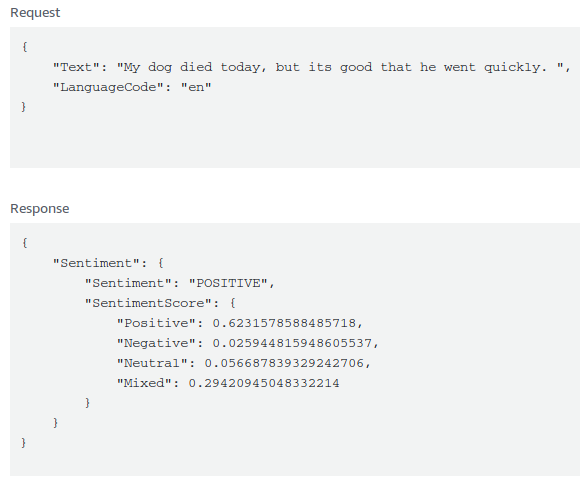
\includegraphics[scale=0.6]{litImgs/comphrendResult.png}
\caption{A display of the input text and incorrect analysis of the sentiment of it by the Amazon Comprehend service}
\label{aws:sentiment}
\end{figure}

\subsubsection{Data Pre-Processing Approaches}

To ensure the input text is in the best format for carrying out sentiment analysis upon, previous work has been analysed to ascertain how this can be optimised.
R. Kim's series on investigating sentiment in Twitter data \cite{towardsDS} has been very influential in this project for inspiring different ways that the data can be pre-processed.
The two main ways that R. Kim's experiment is done is by varying the N-Gram value and number of features supplied to the model.

To preserve the relationship between the words in a sentence, N-grams are very useful since they can help maintain negation of words and helps keep the overall sentiment given in the input sentence better, as shown in Figure \ref{ngrams}. The number of features in this experiment is the $x$ most frequent N-Gram "words" that appear in the dataset.

\begin{figure}[h]
\centering
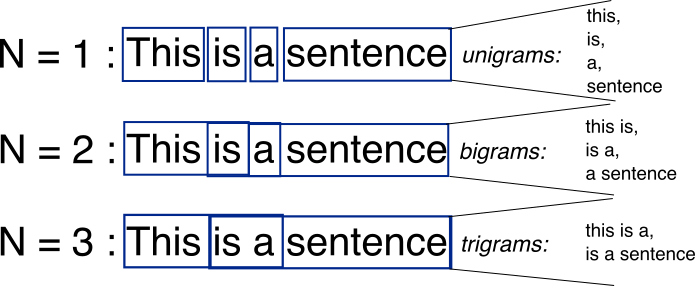
\includegraphics[scale=0.5]{litImgs/ngrams.png}
\caption{Diagram showing the way that the n-grams are created}
\label{ngrams}
\end{figure}

During the experiments put forward by R. Kim, unigrams, bigrams and trigrams are compared and analysed over a feature range of 10000 to 100001. These experiments are done over a totally balanced dataset, with 50\% of the data being classed as having a positive Valence, and the other 50\% with a negative one, and produce results as shown in Figure \ref{towards:DS} that imply that these methods are worth investigating, but can be improved upon.

\begin{figure}[h]
\centering
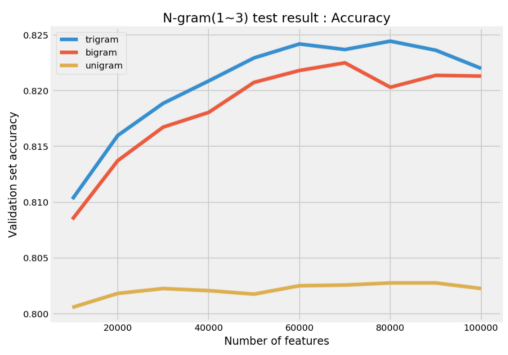
\includegraphics[scale=2.5]{litImgs/towardsDSNgramNFeatures.png}
\caption{Results from R. Kim's investigation over the Sentiment 140 Dataset \cite{go2016sentiment140}}
\label{towards:DS}
\end{figure}

Using these methods, our data flow through the system is now represented in Figure \ref{model:flow}.

\begin{figure}[h]
\centering
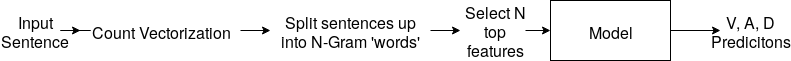
\includegraphics[scale=0.5]{litImgs/modelFlow.png}
\caption{Diagram showing inputs and outputs of the model}
\label{model:flow}
\end{figure}


\pagebreak

\subsubsection{Model building approaches}

A common way of creating a semantic analysis tool is to use movie reviews as mentioned before since these already have numeric values attached to them, or Twitter data due to the sheer volume of text available. Since previous sentiment analysis tools have all been done by training over datasets with the Valence values in discrete variables, Positive and Negative, sometimes with a Neutral class as well, the continuous variables given in the Emobank dataset will be bucketed into classes so that similar methods can be applied. An investigation into finding the optimal number of classes to split the data for each VAD dimension into will be carried out.

When analysing the Valence of tweets, using a lexicon based model, as well as implementing machine learning approaches have been used to great effect \cite{kolchyna2015twitter}, and hence these will be the methods investigated in the the creation of a prediction model.

There has been only a little research into using a multi-dimensional VAD structure to investigate sentiment, one paper primarily explores whether using a VAD structure could be used to help identify burnout in software developers \cite{mantyla2016mining}. In this case, a correlation was found between each of the VAD dimensions and issues raised in messages from the developers, meaning that there is an argument for using multiple dimensions to help understand textual data to a greater degree. An issue with this research is that they only used a word based lexicon where each individual word was assigned a value. This loses the context where which each word is being used, and by using N-Grams this issue will be mitigated.

Before exploring machine learning approaches, a lexicon based model will be established. This is using the bag-of-words dataset \cite{wordsData}, where each individual word in the input sentence is looked up in the dataset, assigned a value, then an average can be taken over the input sentence to give a resultant VAD score. This method has been used before to great effect with binary Valence classification, and so investigating it in this case should lead to promising results \cite{kolchyna2015twitter}.

When choosing the machine learning based classifiers to investigate, literature shows that the same few classifiers such as Logistic Regression and Naive Bayes tend to show the best results for analysing textual data \cite{kolchyna2015twitter} \cite{frank2006naive}.

Logistic Regression is popular due to it being linear and scalable for large datasets \cite{towardsDS}. This is the model that will be initially used for comparing data pre-processing results since it is easy to implement and other work has found it to be the best result for their data. 
Other classifiers that have been shown to give positive results for textual analysis tasks are different styles of Bayes classifiers,  which depend slightly on how many classes are being used. Multinomial is the most common for text categorisation problems, so this one will also be of high interest \cite{frank2006naive}. Support Vector Machines (SVM) have also been used in the past for text classification purposes with a positive results, so these will be incorporated as well \cite{joachims1998text}. Previous work tends to avoid using computationally expensive approaches such as K-Nearest Neighbours and Random Forests due to the size of the datasets being used, but since the Emobank dataset is not that large, it is worth investigating those models as well. To compare these models further, we will also take a note of a rough estimate time it take for each classifier to run, to give us an idea of how much computation each needs.

\subsubsection{Over and Undersampling}

Due to the imbalance of data across the Emobank dataset as shown in Figure \ref{dist:vad}, trying to mitigate the effects of this is a challenge that has different ways of being tackled, and one common way of doing this is through oversampling the minority classes in the data to create a more balanced dataset \cite{towardsDS}.

Since manually inputting more data would take more time than is sensible, the most common way to oversample the data that we are given, is through SMOTE (Synthetic Minority Oversampling Technique). This uses a K-Nearest neighbours approach to create synthetic data of the existing minority samples , and has been shown to have positive results with general machine learning tasks but has been known to be problematic with textual data, due to not actually creating synthetic samples which make logical sense. Investigating this method is worthwhile, although the expected results are fairly unknown as it depends heavily on the data in the minority classes. SMOTE tends to be simpler for continuous data \cite{chawla2002smote}, but we are turning the VAD values into discrete classes so this may lead to more difficulty in creating synthetic samples with accurate VAD scores. Since we will also be applying SMOTE to textual data however, where the synthetic text is likely to not make any sense, the issues caused by this should be minimal in comparison. 

There are other popular oversampling techniques that exist as well, for example just randomly re-sampling the minority class, as well as ADASYN (Adaptive Synthetic Sampling) which is a a form of a SMOTE oversampler which works better for classifiers without clear class boundaries, which will also be investigated.

Another, slightly different approach is to undersample the data, removing less important samples from the majority class so that the dataset is more balanced. This in itself can cause issues since the amount of data that can be trained off is reduced, and literature shows that it tends to not have positive results for textual data, but since it can be used in circumstances when there is not enough data in the minority class to create decent synthetic samples in oversampling, it is worth exploring in this case \cite{more2016survey}. There are different methods of undersampling, from randomly removing items from the majority class, to using the NearMiss undersampler, which uses K-Nearest neighbours to select suitable samples to remove. 

The flow of the data can now be represented by Figure \ref{model:finalFlow}.

\begin{figure}[h]
\centering
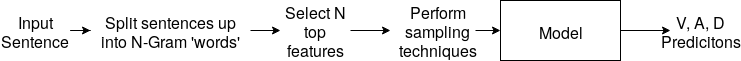
\includegraphics[scale=0.5]{litImgs/finalmodelflow.png}
\caption{Diagram showing the flow of data through the sentiment analysis model including over/undersampling techniques}
\label{model:finalFlow}
\end{figure}

\subsection{Presenting Results}

Existing sentiment analysis tools either do not do anything with a final model, or use the tool as an API for use in general projects \cite{sentimentAPI}.  

To be able to present in the final model in a way that can be used to analyse whether it is useful, an API will be created from it and a web application that can access the data will be produced to allow for further analysis.

Music is also something  that cannot be easily classified into a binary sentimental structure, so relating the output VAD values of the produced model to songs is something that is worth exploring, where a use can be found to directly apply each of the dimensions.

An existing product that does this is the MoodTape web application, which uses the Valence of input text and relates this to the Valence of a song  \cite{moodtape}. Since, as shown in Listing \ref{spotifyJSON}, much more information can be obtained from individual songs than just the Valence, as shown when requesting song data from the Spotify API, an improvement of this project would be to relate the Dominance and Arousal dimensions to some of the other attributes.
\pagebreak
\begin{lstlisting}[style=leftCode, caption={Some of the attributes of a song obtained through requesting information through the Spotify API},captionpos=b, label={spotifyJSON}]
{
    "danceability": 0.322,
    "energy": 0.0593,
    "key": 1,
    "loudness": -53.057,
    "speechiness": 0.0444,
    "acousticness": 0.908,
    "instrumentalness": 0.708,
    "liveness": 0.121,
    "Valence": 0.0165,
    "tempo": 158.402,
    "time_signature": 4
}
\end{lstlisting}

Using a web UI to present the results that has been done in the MoodTape application, and is probably the simplest way to gather all the data together, and so a web application will be produced to provide a basis to answer RQ \ref{RQ2}.

What we can class as "more useful" as can be quite subjective, and as such discussions will be held with test users about how well they believe the predicted song fits them.